\chapter[SCP-106 恐怖老人]{
    SCP-106 The Old Man\\
    SCP-106 恐怖老人
}

\label{chap:SCP-106}

\begin{figure}[H]
    \centering
    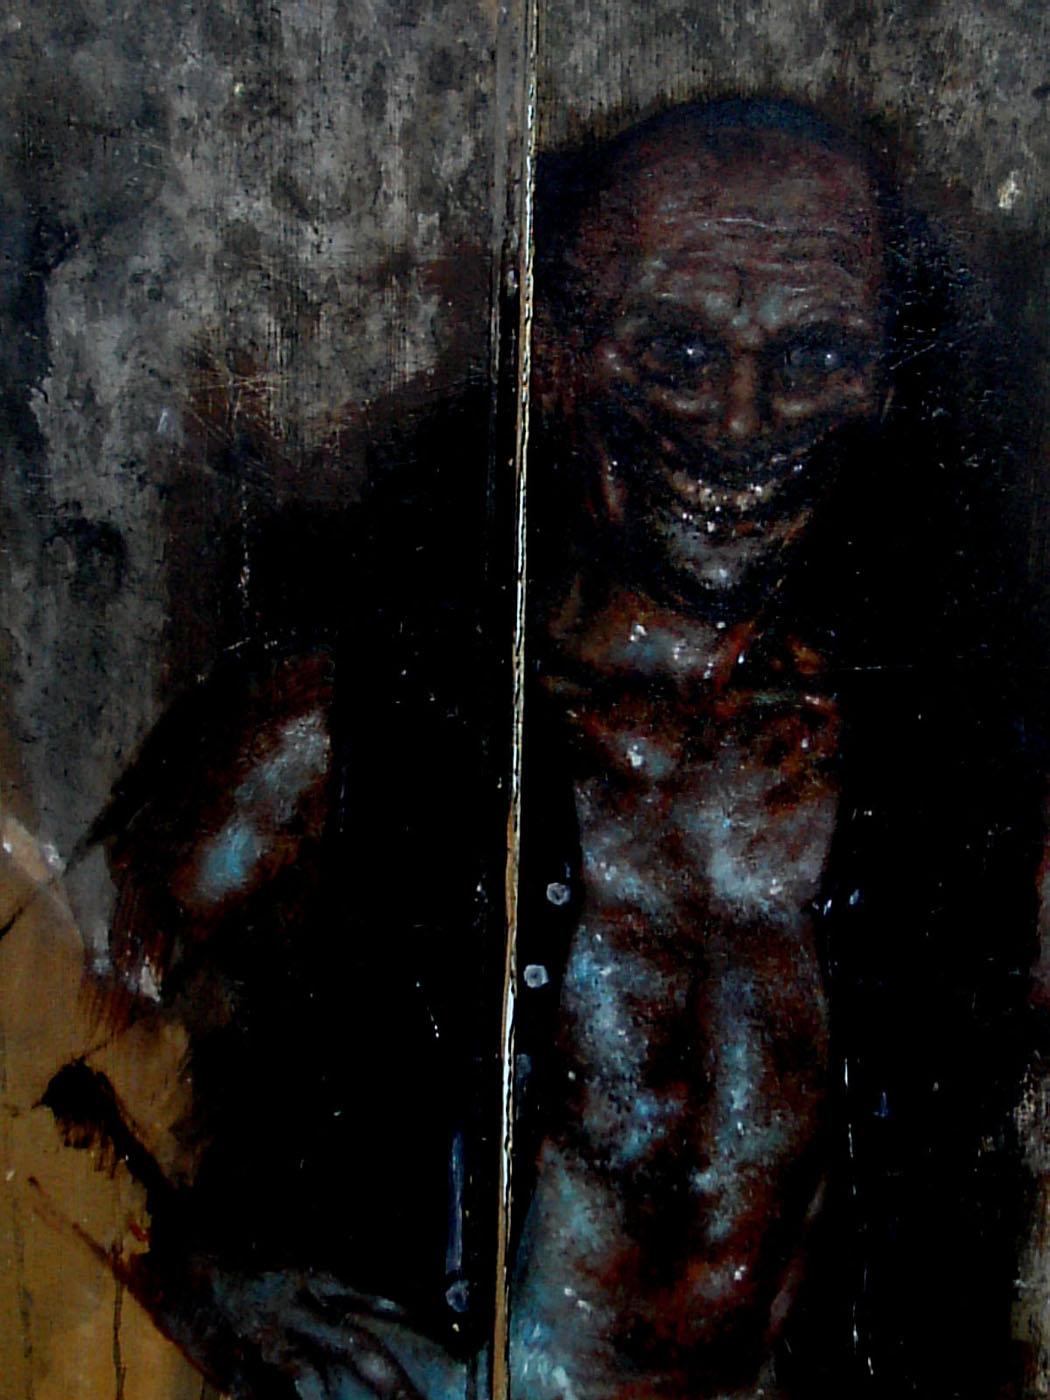
\includegraphics[width=0.5\linewidth]{images/SCP-106.jpg}
    \caption*{SCP-106,出现了一半的形态}
\end{figure}

\bb{项目编号:}SCP-106

\bb{项目等级:}Keter

\bb{特殊收容措施:}

\tred{+ 修订版本 11-6}

\tred{- 修订版本 11-6}

无论何时均禁止与SCP-106的物理接触。所有物理接触必须得到O5议会至少三分之二的投票通过,并仅适用于测试场合。所有人员(研究,安保,D级人员等等)均应与收容隔间保持20米以上距离,除非因维修或重评估检查获得授权。

收容隔间必须悬浮在一个第二隔间之中,其墙壁必须与第一或者叫做“主隔间”的外墙之间保持至少30米。第二隔间必须处于全时的完全监控之下,并且必须持续照明和清理任何碎片。 任何在第二隔间内被注意到的物品,移动,或非正常活动都将导致整个site被封锁。封锁将持续到site指挥发布“情况正常”调度命令为止。

在主隔间,第二隔间,任何员工,或者在SCP-106周围距离200米以内的site中其他位置发生的任何腐蚀现象应立即向site安保上报。任何因SCP-106而失踪的物件或人员将被视为已遗失\slash KIA。任何场合下都不会进行救援尝试。

\ii{注意:SCP-106不存在“温驯”状态。SCP-106任何活动的减少,或服从程度的增加都应视为一种在其积极行动前的诱引策略,并应以此前提处理。}

\mono{警告:SCP有概率逃走}

\tred{+ 修订版本 11-7}

\tred{- 修订版本 11-7}

无论何时均禁止与SCP-106的物理接触。所有物理接触必须得到O5议会至少三分之二的投票通过,并仅适用于测试场合。所有人员(研究,安保,D级人员等等)均应与收容隔间保持30米以上距离,除非site指挥直接下令。

SCP-106被维持在一个密封容器中,具有十六层的衬铅层面板,之间除了最低限度的支撑结构以外应至少以18厘米的开放空间相隔。上述容器通过“恒流系统”在一个液体媒介中保持悬浮。该媒介每24小时进行更换,并持续监测任何“腐蚀”的侵入。

在收容隔间表面,任何员工中,或者在SCP-106周围距离200米以内的site中其他位置发生的任何腐蚀现象应立即向site安保上报。任何因SCP-106而失踪的物件或人员将被视为已遗失\slash KIA。任何场合下都不会进行救援尝试。

SCP-106并不存在“温驯”状态。SCP-106任何活动的减少,或服从程度的增加都应视为一种在其积极行动前的诱引策略,并应以此前提处理。

\ii{注意:观察到SCP-106在穿过铅或者其他类似金属的时候会表现出轻微的"抵触感"。材料的厚度似乎没有影响。此外,多层的薄质材料大致会“减慢”SCP-106,使其需要穿入再穿出。液体也能够暂时“扰乱”SCP-106.}

\mono{NOTE: SCP DISCONTINUED DUE TO MULTIPLE SURFACE BREACHES. AGITATION SYSTEM CONTINUED TO DISPERSE CORROSION DURING BREACH EVENT, RESULTING IN MULTIPLE BREACHES AND FULL CONTAINMENT FAILURE}

\bb{重编版本11-8}

任何时候的都不得与106进行任何物理性接触。所有的物理性接触都需要05级人员之中三分之二以上投票同意。所有这些接触都必须在AR-II最大安全站点之中进行,并且要在一般的非必要人员进行撤离之后。所有人员(包括研究人员、安全人员、D级人员等。)必须在任何时候都离收容房间60m以上,除非是在收容失效事件之中。

SCP-106被收容在一个上锁的房间之中,该房间是由衬铅钢组成。该房间必须被封锁于40层完全相同的材料之中,每一层材料之间都必须要有不少于36cm的间隔。层与层之间的支撑架必须随机排列。该房间必须用ELO-IID电磁支持使之悬浮在离任何表面距离不低于60cm处。

第二层收容场所应该由16个球形“房间”组成,每一个之中都用不同的液体充满并且布满了随机的支撑架和支撑表面。第二层收容场所应该装配满灯光系统,使得该收容区域之中能够在不需要人员介入的情况下始终保持能够立刻充满不低于80000流明的光。2个收容区域都应该保持24小时的不间断监视。

如果观察到了在任何收容区域表面的任何腐蚀斑痕,工作人员,或者是在离106房间200范围以内的人员应该马上向站点安全处报告。任何因为106而失去的人员或者物体都将会被认为是失踪\slash 阵亡,并且不会有任何的援救尝试。

\ii{注释:一直持续的研究表明,当面对复杂\slash 随机排布的建筑结构时,SCP-106将会被“扰乱”,将会对于出入以上结构感到明显的犹疑不决。SCP-106还显示出了一种对于突然的强光的厌恶感。这将不会对106造成任何物理性损伤,但是会导致他迅速地回到在固体表面开出的“口袋次元”之中。}

\ii{这些观察,包括它对于铅的厌恶和对于液体的困惑,已经将其破坏收容的几率下降到了43\%。那个“初级”牢房同时也方便在再收容事件之中使用再收容协议██ -███ -█,观察仍在进行之中。}

\bb{描述:}

\begin{figure}[H]
    \centering
    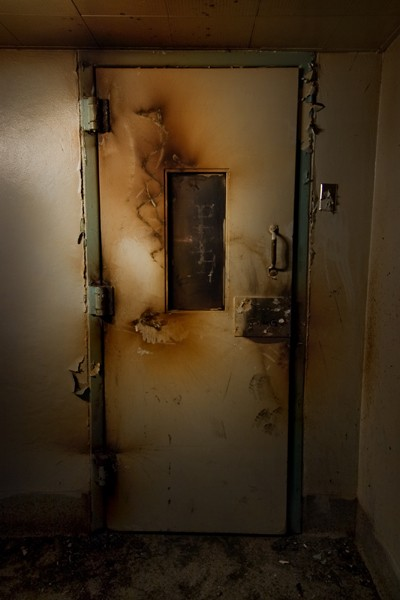
\includegraphics[width=0.5\linewidth]{images/SCP-106-2.jpg}
    \caption*{在最初的收容牢房上造成的腐蚀,特殊收容措施在那之后进行了重编。}
\end{figure}

SCP-106表现出了一个老年人类男子的外形,通常有着高度腐烂的外形。他的外形经常发生改变,但是那“腐烂”程度被观察到了各种各样的形式。SCP-106并不是十分灵敏,并且也会一天之中一动不动,等待着猎物。SCP-106同样也可以使任何的垂直表面剥落并且可以以不确定的方式上下倒挂着。106将会试着使其猎物无力化,通常通过攻击主要器官、肌肉组织或者腿部来实现这一点,然后将残疾的猎物拖入它的口袋空间之中。SCP-106看起来更喜欢将在10-25年龄区段的人类作为其猎物。

106能够对其触碰的固体导致一种“腐蚀”效应,在触碰数秒之后导致物质的物理性崩溃。材料会被观察到生锈、腐朽和最终崩溃的过程,并且会创造出一种黑色的、像黏液一样类似于包裹着106的物质的材料。这种效应对于生命物体特别有害,并且这被认为是一种“消化前”行为。这种腐蚀效应将会在触碰之后持续6个小时,在那之后这效应看起来就“烧尽”了。

106能够穿过固体物质,在它身后留下一大段的腐蚀性粘液。106能够“消失”在固体物质之中,进入一种被假定为“口袋次元”的物质之中。106接下来能够通过与任何它最初进入的固体物质相连的固体物质出去(例如:“进入”房间的内墙,从外墙“出去”。进入一堵墙壁,从天花板离开)。这现在还不知道是否是106原型的关键,或者说只是它制造出来的“巢穴”。

对于“口袋次元”有限的观察显示它是由房间和大厅组成的,有着{[}数据删除]的入口。这种活动能够持续“数日”,并且会有一些项目被释放出来,很明显是出于狩猎、回收或者是{[}数据删除]的目的。

\begin{figure}[H]
    \centering
    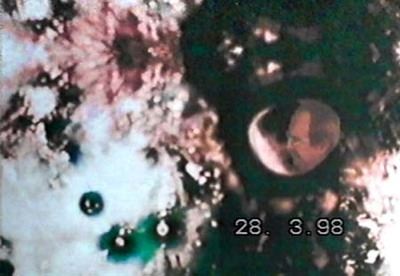
\includegraphics[width=0.5\linewidth]{images/SCP-106-3.jpg}
    \caption*{从一名猎物身上所携带的摄像机上传回的图像,摄像机在猎物被绑走之后2天之后在一个大厅之中被回收,环境未知。}
\end{figure}

\hr

\bb{附录:}

\bb{SCP评估注释:}

因为106极度难以收容的自然特性,106每三个月或是在一次收容失效之后都要进行一次评估。物理性的拘束是不可能的,而直接的物理性伤害看起来对于106没有什么作用。现阶段该SCP,出于██\slash ██\slash ████事件的原因,需要持续不断的基本监视和迅速的反应机制。事先地,更为有前瞻性的特殊收容措施现在正被征集着,这是因为██,███,██,█和████的收容破坏事件。

\bb{行为注释:}

106看起来要经历很长一段时间的“休眠”,在该阶段之中它会完全不动最多3个月。引发这种现象的原因现在未知;但是,已经证明这是一种“哄骗”策略,106会从这种状态之中转换成一种十分好战的状态。并且会攻击和绑架人员,对其收容房间和站点造成大量恶劣的伤害。再收容协议{[}数据删除]。

106的捕食行为看起来是由欲望驱使的,而不是饥饿感。106会再一次捕猎之中攻击并收集数个猎物,长时间在它的“口袋次元”之中保持着“活着”的猎物。106没有表现出一种可以被确定的“极限”,并且在一次捕猎行动之中会猎取随机数量的猎物。

那个由106通过的次元似乎只能由106进入。记录设备和传输设备看起来在那个次元之中也能工作,但是数据质量有明显的下降。它显示106会与猎物“玩耍”,并且表现出可以控制那个次元之中的空间、时间以及知觉。106表现出了{[}数据删除]。

\bb{再收容协议██ -███ -█:}

在106造成的收容破坏事件之中,一名在10-25岁年龄区间之中的人员应被准备好来进行收容,他被安置在一个重新代替使用的收容牢房之中。当这个牢房准备完毕之后,作为诱饵的人员将会被伤害,最好能是伤害一条主要的长骨的方式,比如说大腿骨,或者是一条主要的腿骨,比如说阿基里斯腱。被伤害的人员应被放置在准备好的牢房之中,并且上述人员所发出的声音将会通过广播系统传播出去。

\begin{figure}[H]
    \centering
    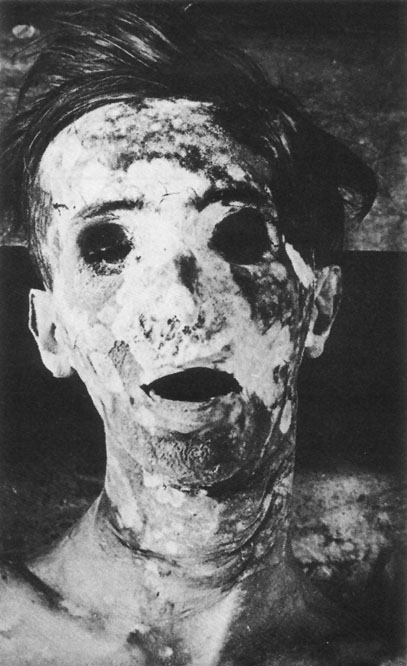
\includegraphics[width=0.5\linewidth]{images/SCP-106-4.jpg}
    \caption*{█████特工,在被106释放了之后的状态,该人员失踪了2个小时,并且在被释放之后活了1个小时。}
\end{figure}

106通常都会在听到诱饵的声音5-10分钟之后被诱饵所吸引。如果106对于一开始的广播没有做出反应,每20分钟都应给予诱饵更多的创伤直到106做出了回应。数名诱饵在严重的收容失效事件之中可以被使用。

106通常都会在捕食了一名诱饵之后进入休眠状态。顺便一说,该人员将会{[}数据删除]。
